\begin{figure}[ht]
\ffigbox
	{\begin{subfigure}[b]{0.48\linewidth}
		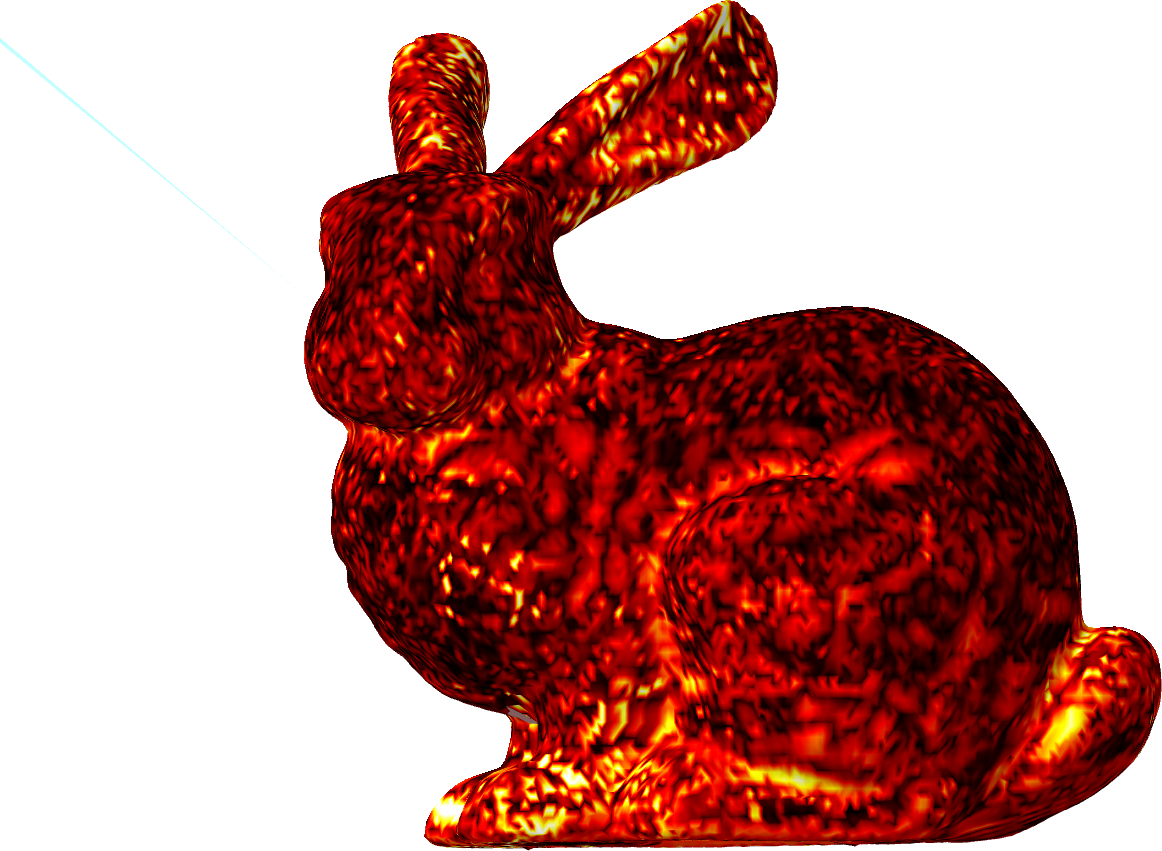
\includegraphics[width=1.0\linewidth,height=0.3\textheight,keepaspectratio]{data/acquired_meshes/bun_zipper_edited_r1_n4_v256_funcvals_0iter.png}
		\caption{Stanford Bunny 0iter}\label{fig:bun.a}
	\end{subfigure}
	\begin{subfigure}[b]{0.48\linewidth}
		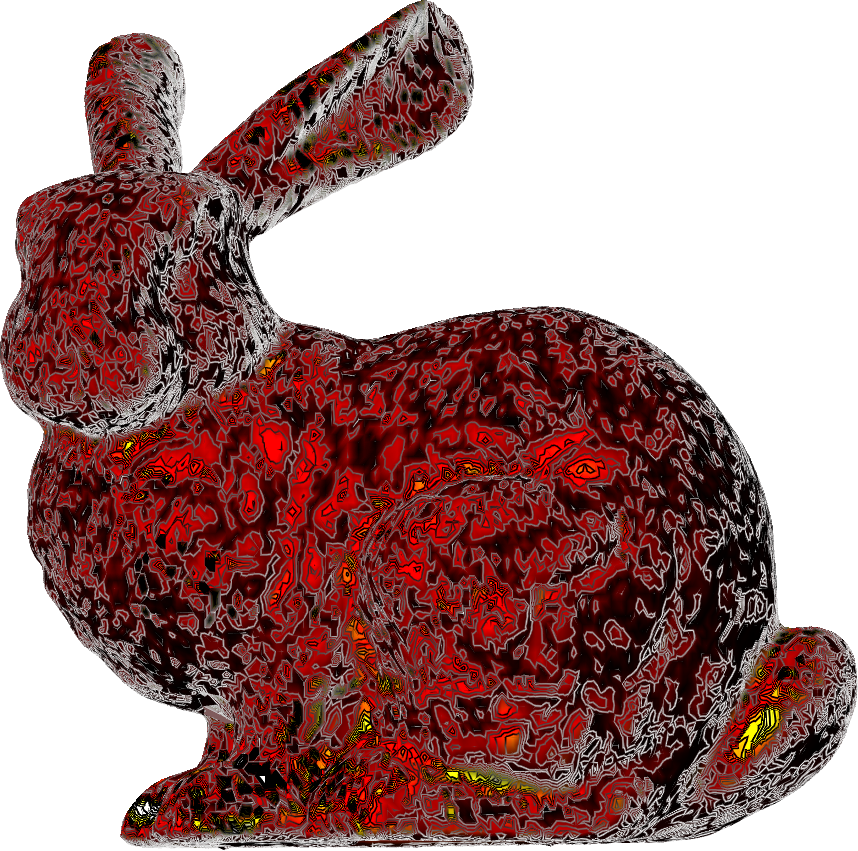
\includegraphics[width=1.0\linewidth,height=0.3\textheight,keepaspectratio]{data/acquired_meshes/bun_zipper_edited_r1_n4_v256_funcvals_isolines_0iter.png}
		\caption{Stanford Bunny 0iter isolines}\label{fig:bun.b}
	\end{subfigure}

	\bigskip
	\begin{subfigure}[b]{0.48\linewidth}
		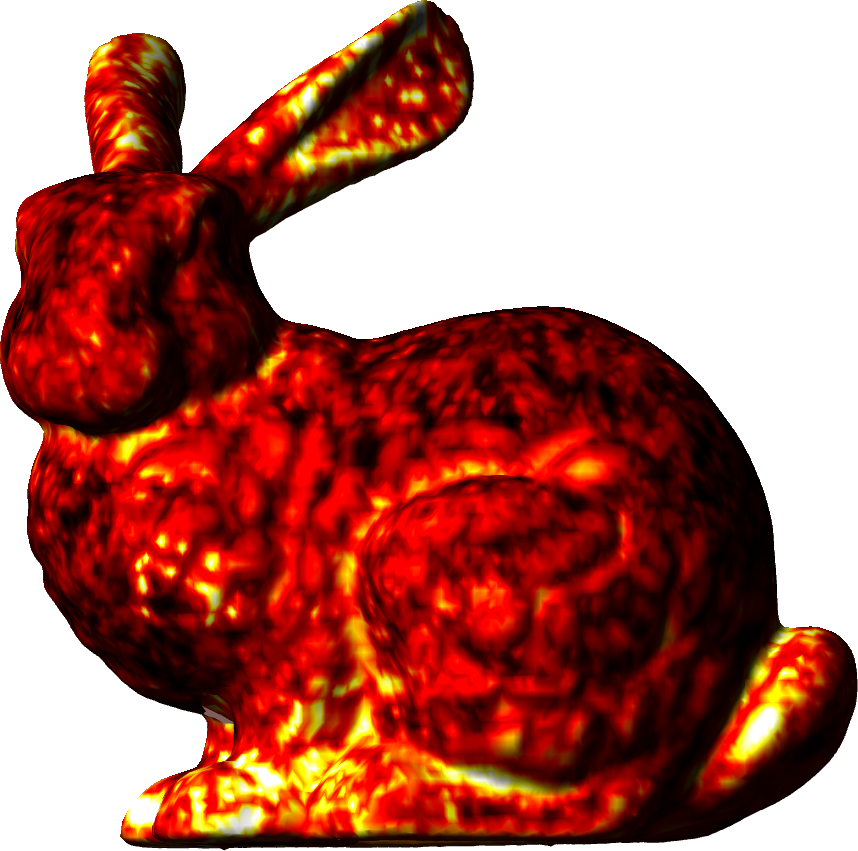
\includegraphics[width=1.0\linewidth,height=0.3\textheight,keepaspectratio]{data/acquired_meshes/bun_zipper_edited_r1_n4_v256_funcvals_10iter.png}
		\caption{Stanford Bunny 10iter}\label{fig:bun.c}
	\end{subfigure}
	\begin{subfigure}[b]{0.48\linewidth}
		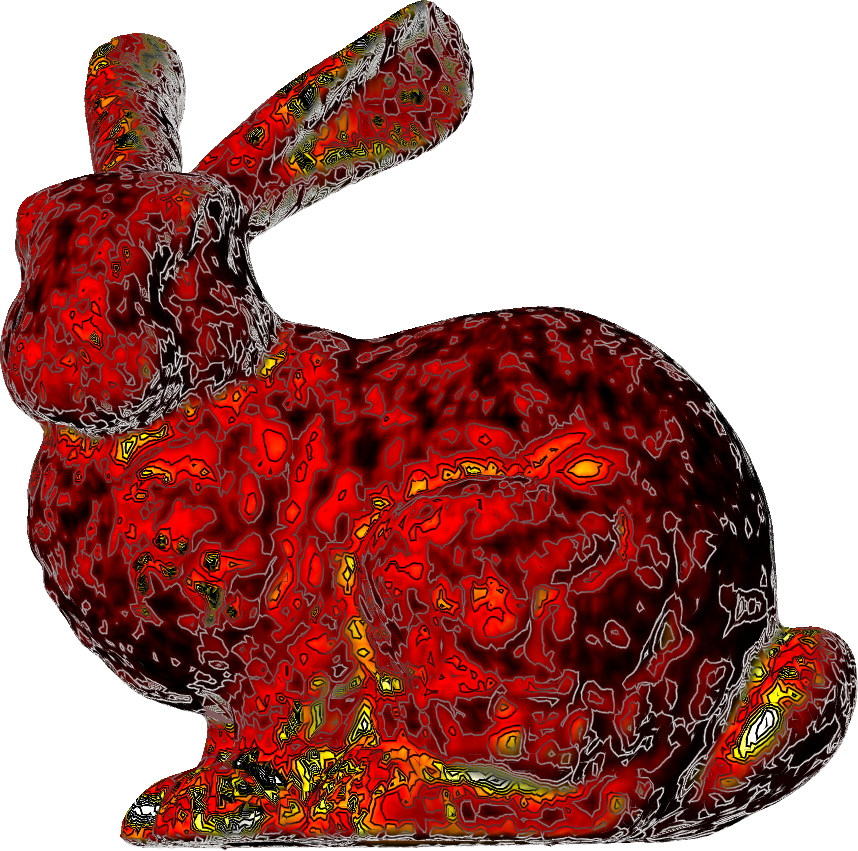
\includegraphics[width=1.0\linewidth,height=0.3\textheight,keepaspectratio]{data/acquired_meshes/bun_zipper_edited_r1_n4_v256_funcvals_isolines_10iter.png}
		\caption{Stanford Bunny 10iter isolines}\label{fig:bun.d}
	\end{subfigure}

	\bigskip
	\begin{subfigure}[b]{0.48\linewidth}
		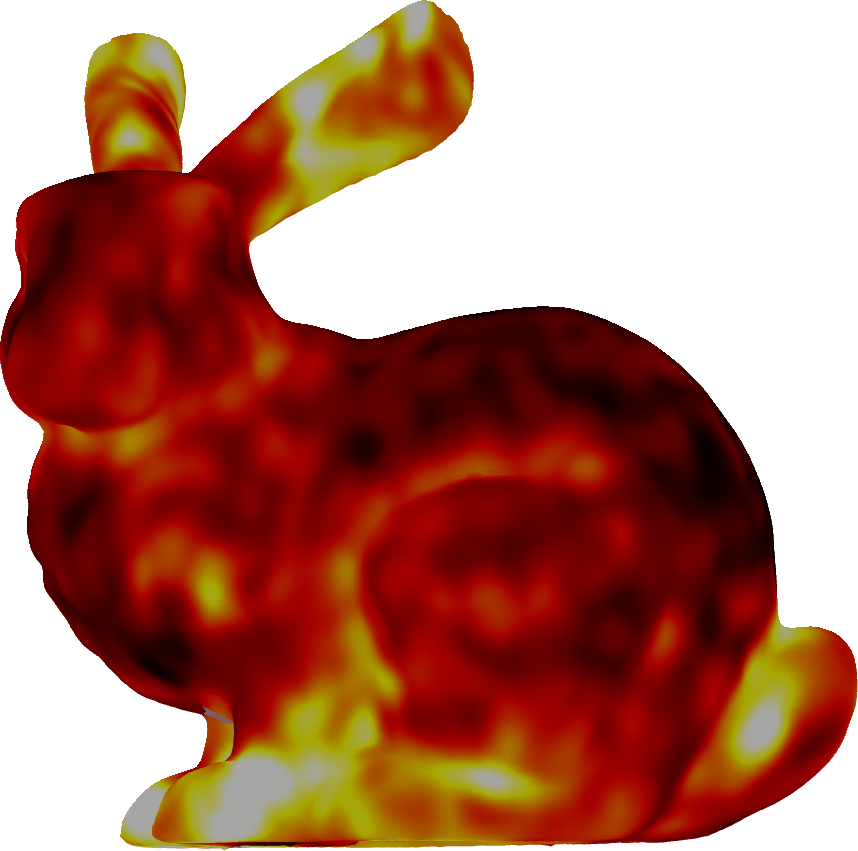
\includegraphics[width=1.0\linewidth,height=0.3\textheight,keepaspectratio]{data/acquired_meshes/bun_zipper_edited_r1_n4_v256_funcvals_100iter.png}
		\caption{Stanford Bunny Wireframe}\label{fig:bun.e}
	\end{subfigure}
	\begin{subfigure}[b]{0.48\linewidth}
		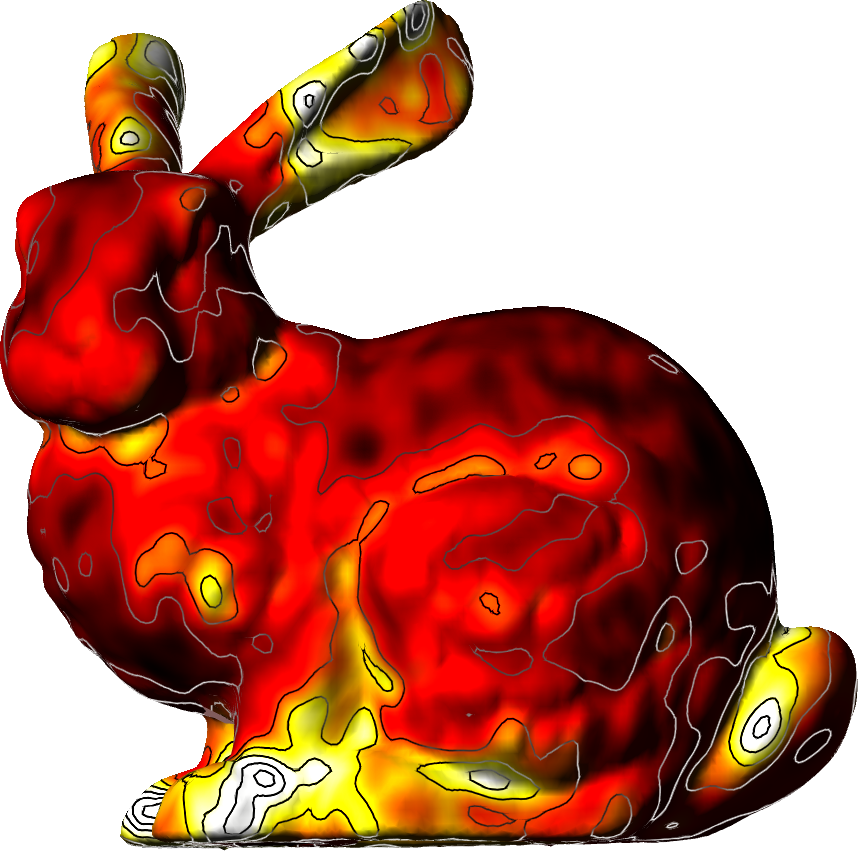
\includegraphics[width=1.0\linewidth,height=0.3\textheight,keepaspectratio]{data/acquired_meshes/bun_zipper_edited_r1_n4_v256_funcvals_isolines_100iter.png}
		\caption{Stanford Bunny 100iter isolines}\label{fig:bun.f}
	\end{subfigure}}
	{\caption[Stanford Bunny]{Stanford Bunny\ldots}\label{fig:bun}}
\end{figure}
